%! alt The plane through line PQ and the point A, after B has been rotated about line PQ into this plane, onto the side away from A, to the point B'. P and Q lie on the line 8 apart. A is 3 from the line with foot P, and B' is 7 from the line with foot Q, both at right angles. The straight segment AB' crosses the line at X, and AB' squared is 8 squared plus 10 squared, which is 164.
%! after_paragraph 4
%! scale 2/5
% The shared preamble of every Cevian figure. pipeline/figures turns these colours into theme-aware paint,
% and refuses any other colour, so draw only with them:
%   figink (lines and labels), figaux (construction lines), figaccent (the object the argument turns on),
%   figtint and figaccenttint (light fills).
\documentclass[border=1.5pt]{standalone}
\usepackage{tkz-euclide}
\definecolor{figink}{RGB}{0,0,0}
\definecolor{figaux}{RGB}{85,85,85}
\definecolor{figaccent}{RGB}{192,57,43}
\definecolor{figtint}{RGB}{221,221,221}
\definecolor{figaccenttint}{RGB}{245,213,208}
% tkz-euclide's defaults draw circles, compasses and marks in 50% grey and fill points with a tint.
\makeatletter
\def\tkz@otherlinecolor{figink}
\def\tkz@euc@circlecolor{figink}
\def\tkz@euc@compasscolor{figink}
\def\tkz@euc@mkcolor{figink}
\def\tkz@mk@fill{figink}
\def\tkz@euc@pointfillcolor{figink}
\makeatother
\tkzSetUpLine[color=figink,line width=.7pt]
\tkzSetUpArc[color=figink,line width=.7pt]
\tkzSetUpCompass[color=figink,line width=.5pt]
\tkzSetUpPoint[color=figink,fill=figink,size=3.1pt]
\tikzset{
  every picture/.style={line cap=round,line join=round,color=figink},
  circle style/.append style={color=figink,line width=.7pt},
  aux/.style={color=figaux,line width=.45pt,dash pattern=on 2.6pt off 2pt},
  key/.style={color=figaccent,line width=1pt},
  mk/.style={color=figink,line width=.5pt},
  lbl/.style={color=figink,inner sep=2.2pt},
  len/.style={color=figink,inner sep=1.5pt,font=\small},
}

\begin{document}
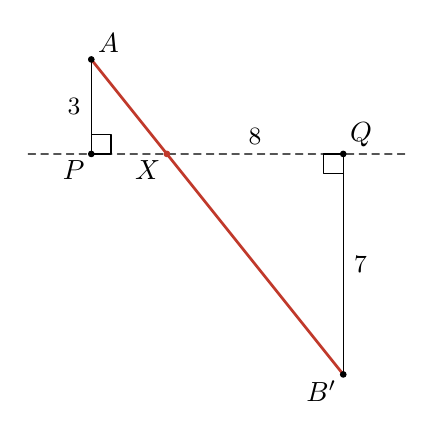
\begin{tikzpicture}
\tkzDefPoint(0.0,0.0){P} %! P = (0, 0)
\tkzDefPoint(3.2000000,0.0){Q} %! Q = (8, 0)
\tkzDefPoint(0.0,1.2000000){A} %! A = (0, 3)
\tkzDefPoint(3.2000000,-2.8000000){Bp} %! Bp = (8, -7)
\tkzDefPoint(0.96000000,0.0){X} %! X = (12/5, 0)
\tkzDefPoint(-0.80000000,0.0){L1} %! L1 = (-2, 0)
\tkzDefPoint(4.0000000,0.0){L2} %! L2 = (10, 0)
\tkzDefPoint(-0.22000000,0.60000000){N3} %! N3 = (-0.55, 1.5)
\tkzDefPoint(3.4200000,-1.4000000){N7} %! N7 = (8.55, -3.5)
\tkzDefPoint(2.0800000,0.22000000){N8} %! N8 = (5.2, 0.55)
%! fact dist(P, Q) == 8
%! fact dist(P, A) == 3
%! fact dist(Q, Bp) == 7
%! fact perp(A, P, P, Q)
%! fact perp(Bp, Q, P, Q)
%! fact collinear(X, A, Bp)
%! fact on_segment(X, P, Q)
%! fact equal(dist(A, Bp)**2, 164)
\tkzDrawSegment[aux](L1,L2)
\tkzDrawSegments(P,A Q,Bp)
\tkzDrawSegment[key](A,Bp)
\tkzMarkRightAngle[size=.25,mk](A,P,Q)
\tkzMarkRightAngle[size=.25,mk](Bp,Q,P)
\tkzDrawPoints(P,Q,A,Bp)
\tkzDrawPoints[color=figaccent,fill=figaccent](X)
\tkzLabelPoint[below left,lbl](P){$P$}
\tkzLabelPoint[above right,lbl](Q){$Q$}
\tkzLabelPoint[above right,lbl](A){$A$}
\tkzLabelPoint[below left,lbl](Bp){$B'$}
\tkzLabelPoint[below left,lbl](X){$X$}
\tkzLabelPoint[anchor=center,len](N3){$3$}
\tkzLabelPoint[anchor=center,len](N7){$7$}
\tkzLabelPoint[anchor=center,len](N8){$8$}
\end{tikzpicture}
\end{document}
